%



% \chapter{Results}
% This section presents the main findings of the project

% \pdfcomment{Compare the effect of other physical or atmospheric variables on the error, like include an entire section}
% \pdfcomment{Add a point density per sqaure meter for each site}
% \pdfcomment{average depth for each site?}
% \pdfcomment{how many transects actually had data?}
% % \section{Random Sampling vs sampling along lines}

% \section{Petten Test Site}
% Most research results show that spaceborne lidar is not effective at retrieving bathymetry from very turbid waters. To test the upper limits of this, ICESat-2 data for the coast of Petten, NL was downloaded. As expected, there was no bathymetric signal found, likely due to the inability of the laser to penetrate the turbid water.

% However, The Dutch government provides a dataset of point surveys of the Dutch coast. This data was used as input to the kriging and Kalman updating code.

% \subsection{Site Conditions Summary}
% \begin{table}[h!]
%     \begin{minipage}{0.5\textwidth}
%         \centering\begin{tabular}{r l }
%             Parameter                                                 & \textbf{Value}                  \\
%             \hline
%             Location                                                  &                                 \\
%             Tidal Range \footcite{Tidal_data_reanalysis2022}          & \qty{2.24}{m}                   \\
%             Average Secchi Depth \footcite{ACRI-STGlobColourTeam2020} & \qty{3.86}{m}                   \\
%             Validation Data vertical RMS error                        & \qty{}{m} \pdfcomment{look up}  \\
%             Validation Data Horizontal Resolution                     & \qty{}{m} \pdfcomment{look up?} \\
%             Vertical Datum                                            & Normaal Amsterdams Peil (NAP)   \\
%         \end{tabular}
%     \end{minipage}
%     \caption{Site conditions for the Florida Keys site}
%     \label{table:Pettensitestats}
% \end{table}

% \subsection{Validation data}
% The validation data for this site was from a 2021 survey performed by Van Oord.
% \subsection{Error Jarkus Vs. Survey}
% There was some error between the Jarkus survey points and the Van Oord 1m surveyed grid. The error metrics are shown in table \ref{tab:jarkus_vs_survey_error}, and the distribution of the error is shown in figure
% \begin{table}[h!]
\caption{Error between Surveyed Bathymetry grid and Jarkus}
\label{tab:jarkus_vs_survey_error}
\begin{tabular}{lrr}
\toprule
 & MAE & RMSE \\
\midrule
Petten & 0.267152 & 0.439663 \\
\bottomrule
\end{tabular}
\end{table}


% \begin{figure}[h]
%     \centering
%     \includegraphics[width=0.5\textwidth]{figures/Petten_lidar_estimated_vs_truth.jpg}
%     \caption{Jarkus Survey points vs same location on Van Oord Survey data}
%     \label{fig:jarkus_vs_survey}
% \end{figure}

% \subsection{Jarkus Data kriging and Kalman update}
% \begin{table}[h!]
\caption{Improvement in Error when incorporating Kriged Jarkus data}
\label{tab:jarkus_kriging_kalman_error}
\begin{tabular}{lrr}
\toprule
 & RMSE & MAE \\
\midrule
Naive Bilinear Interpolation & 1.473726 & 1.311282 \\
Kalman Updated Raster & 0.722669 & 0.483035 \\
Kriged Raster & 0.743263 & 0.496904 \\
\bottomrule
\end{tabular}
\end{table}



% \section{Marathon Key Test Site}
% The area surrounding Marathon Key in the Florida Keys in Florida, USA. The area has a wide shelf, a microtidal tidal environment, and very clear water, so it is an ideal site to apply this methodology. 

% \begin{table}[h]
%     \begin{minipage}{0.5\textwidth}
%         \centering\begin{tabular}{r l }
%             Parameter                                                      & \textbf{Value}                                 \\
%             \hline
%             Location                                                       & -81.04472,24.72868                             \\
%             Tidal Range \footcite{Tidal_data_reanalysis2022}               & \qty{0.51}{m}                                  \\
%             Average Secchi Depth \footcite{ACRI-STGlobColourTeam2020}      & \qty{0.0}{m}                                   \\
%             Validation Data Vertical RMS error \footcite{Keys2019Lidar}    & \qty{0.056}{m}                                 \\
%             Validation Data Horizontal Resolution \footcite{Keys2019Lidar} & \qty{9.4e-6}{ \degree} $\approx$ \qty{0.95}{m} \\
%             Vertical Datum \footcite{Keys2019Lidar}                        & local MSL                                      \\
%         \end{tabular}
%     \end{minipage}
%     \caption{Site conditions for the Florida Keys site}
%     \label{table:floridasitestats}
% \end{table}


% \subsection{ICESat-2 Transects within AOI}
% The AOI used the validate the method is shown in figure \ref{fig:keys_transects} below.
% \begin{figure}[h]
%     \centering
%     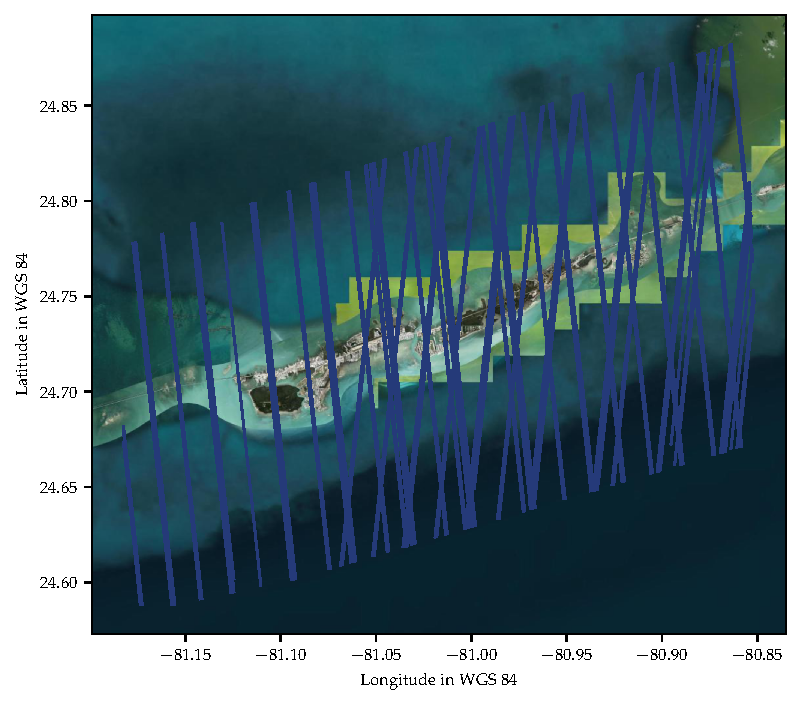
\includegraphics[width=0.5\textwidth]{figures/florida_keys_tracklines.pdf}
%     % \input{figures/study_site_tracklines.pgf}
%     \caption{Location of ICESat-2 Transects in Florida keys Study Area}
%     \label{fig:keys_transects}
% \end{figure}
% \subsection{Validation Data}
% The validation data used for this site is from a detailed lidar survey of the area performed in 2018 and 2019 by Quantum Spatial, Inc. \parencite{Keys2019Lidar}. The survey was performed using a Riegl VQ-880-G hydrographic airborne laser scanner. The instrument is designed for high bathymetric accuracy in shallow water.
% %removing validation data for now, maybe replace this with a contour map 
% % \begin{figure}[h]
% %     \centering
% %     \includegraphics[width=\textwidth]{figures/florida_keys_ras.jpg}
% %     \caption{Ground Truth topobathymetric Survey taken after Hurricane Irma}
% %     \label{fig:truebathy}
% % \end{figure}
% \subsection{Error in lidar photon data}

% % \begin{table}
\caption{Atmospheric Profile vs error}
\begin{tabular}{lr}
 & 0 \\
atm_profile &  \\
profile_1 & 0.524872 \\
profile_2 & 0.666805 \\
profile_3 & 0.551757 \\
\end{tabular}
\end{table}


% % \begin{table}
\caption{Beam Strength vs Error}
\begin{tabular}{lr}
 & RMS error \\
beamtype &  \\
strong & 11.206860 \\
weak & 9.363623 \\
\end{tabular}
\end{table}


% \subsection{Bathymetric photons}
% Figure \ref{fig:bathyphotonmap} shows the location and estimated bathymetric depths of individual ICESat-2 photon returns.
% \pdfcomment{change colorbars to match}
% \begin{figure}[h]
%     \centering
%     \includegraphics[width=\textwidth]{figures/Florida_keys_photon_map.pdf}
%     \caption{Geographic distribution of Bathymetric photon data}
%     \label{fig:bathyphotonmap}
% \end{figure}

% \subsection{Lidar updated GEBCO vs. Simple bilinear Interpolation}
% The results when comparing a raw interpolation of GEBCO to
% % \begin{table}[h!]
\caption{Comparison of the error metrics between the Kalman updating and a simple bilinear interpolaton of GEBCO data}
\label{raster_rmse_comparison}
\begin{tabular}{lrr}
\toprule
 & RMSE & MAE \\
\midrule
Naive Bilinear Interpolation & 2.086102 & 0.986900 \\
Kalman Updated Raster & 1.345899 & 0.836557 \\
\bottomrule
\end{tabular}
\end{table}

% \begin{table}
\centering
\caption{Improvement in error metrics after applying Kalman Updating of kriged data}
\label{tab:florida_keys_gebco_raster_error}
\begin{tabular}{lrr}
\toprule
 & RMSE & MAE \\
\midrule
Naive Bilinear Interpolation & 2.21 & 1.11 \\
Kalman Updated Raster & 1.41 & 0.85 \\
Kriged Raster & 2.28 & 1.31 \\
\bottomrule
\end{tabular}
\end{table}



% \section{St. Croix}

% \subsection{Site Characteristics}

% St. Croix is in the US Virgin Islands. \pdfcomment{flesh out}

% \begin{figure}[h]
%     \centering
%     \includegraphics[width=\textwidth]{figures/Stcroix_tracklines.pdf}
%     \caption{ICESat-2 tracklines available in the St. Croix site}
%     \label{fig:st-croix-tracklines}
% \end{figure}

% \subsection{ICESat-2 Signal Extraction}
% After downloading the above tracklines and processing them, the points shown in were identified by the algorithm as containing bathymetric measurements.

% \begin{figure}[h]
%     \centering
%     \includegraphics[width=\textwidth]{figures/Stcroix_photon_map.pdf}
%     \caption{Point estimates of bathymetry from KDE algorithm }
%     \label{fig:stcroix-bathy-points}
% \end{figure}

% This site showed excellent agreement between the point ICESat-2 estimated lidar and the validation data. The error metrics are shown in table \ref{tab:stcroix_lidar_error}

% \begin{table}[h!]
\caption{Error between the point bathymetry and ground-truth data}
\label{tab:stcroix_lidar_error}
\begin{tabular}{lrrrrr}
\toprule
 & MAE & RMSE & Median Abs error & R2 Score & Average Error \\
\midrule
stcroix & 0.299882 & 0.545965 & 0.176959 & 0.975837 & -0.087435 \\
\bottomrule
\end{tabular}
\end{table}


% \subsection{GEBCO Updating}

% The change in the error metrics that is provided by the  is shown in table \ref{tab:stcroix-raster-error}

% \begin{table}
\centering
\caption{Improvement in error metrics after applying Kalman Updating of kriged data}
\label{tab:stcroix_gebco_raster_error}
\begin{tabular}{lrrr}
\toprule
 & RMSE [m] & MAE [m] & Mean Error [m] \\
\midrule
Naive Bilinear Interpolation & 6.45 & 4.30 & -1.01 \\
Kriged Raster & 6.79 & 4.10 & -2.91 \\
Kalman Updated Raster & 4.63 & 3.20 & -1.14 \\
\bottomrule
\end{tabular}
\end{table}


% \section{Charlotte Amalie}
% Another test site is the island of Charlotte Amalie in the US Virgin Islands. Basic details about the test site are in \ref{table:charlotteamalie_datatable}
% \begin{table}[h]
%     \begin{minipage}{0.5\textwidth}\pdfcomment{fill in table}
%         \centering\begin{tabular}{r l }
%             Parameter                                                 & \textbf{Value} \\
%             \hline
%             Location                                                  &                \\
%             Tidal Range \footcite{Tidal_data_reanalysis2022}          & \qty{}{m}      \\
%             Average Secchi Depth \footcite{ACRI-STGlobColourTeam2020} & \qty{}{m}      \\
%             Validation Data vertical 95\% confidence                  & $x$ m          \\
%             Validation Data Horizontal Resolution                     & \qty{}{m}      \\
%             Vertical Datum                                            & lookup         \\
%         \end{tabular}
%     \end{minipage}
%     \caption{Site conditions for the Charlotte Amalie}
%     \label{table:charlotteamalie_datatable}
% \end{table}
% Overall there where X \pdfcomment{lookup number of transects} transects of ICESat-2 data available for the site, and their distribution is shown in figure \ref{fig:charlotteamalietracklines}.

% \begin{figure}[h]
%     \centering
%     \includegraphics[width=\textwidth]{figures/Charlotteamalie_tracklines.pdf}
%     \caption{ICESat-2 tracks in the Charlotte Amalie Test site}
%     \label{fig:charlotteamalietracklines}
% \end{figure}

% \subsection{Lidar Points found for site}
% Figure \ref{fig:pointmapcharlotteamalie} shows the geographic distribution of the points

% \begin{figure}[h]
%     \centering
%     \includegraphics[width=\textwidth]{figures/Charlotteamalie_photon_map.pdf}
%     \caption{Charlotte Amalie points}
%     \label{fig:pointmapcharlotteamalie}
% \end{figure}

% The error for the site is shown in \ref{fig:charlotteamalie-lidar-bias}

% \begin{figure}[h]
%     \centering
%     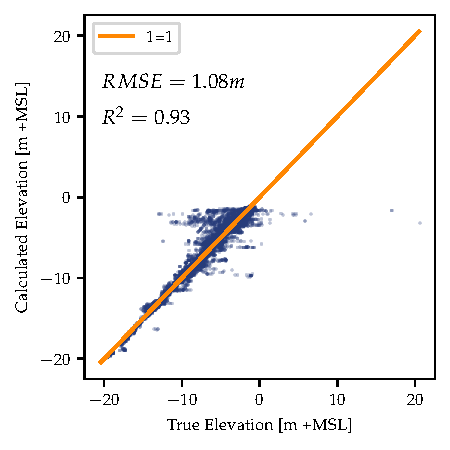
\includegraphics[width=0.5\textwidth]{figures/charlotteamalie_lidar_estimated_vs_truth.pdf}
%     \caption{Bias plot showing the agreement between the validation data and the lidar points for Charlotte Amalie}
%     \label{fig:charlotteamalie-lidar-bias}
% \end{figure}


% \section{Oahu}
% One test site that was selected based on the clear water and the high quality validation data is the Island of Oahu, in the US state of Hawai'i. The island has an extremely varied shelf and coastal environment along its length, to it provides the ability to test the results in in areas with a variety of offshore slopes and wave energy environments.

% Because of the size of the island, the nearshore zone was divided into 8 different zones, for which the data was downloaded and processed seperately. The results were then combined and summarized. A map of the area that shows the available ICESat-2 tracklines and the subareas used to download the and process the data are shown in figure \ref{fig:oahu-all-sites-transects}

% \begin{figure}[h]
%     \centering
%     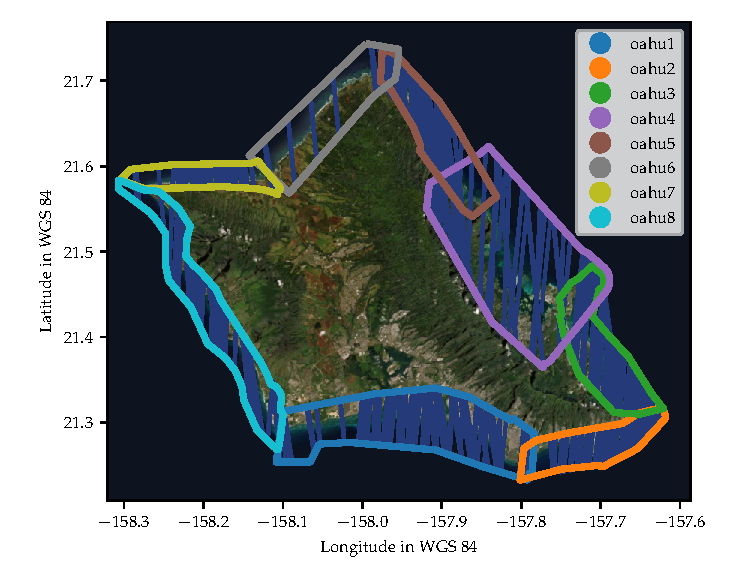
\includegraphics[width=\textwidth]{figures/Oahu_all_tracklines.pdf}
%     \caption{Transects and subsite distribution for Oahu Test site}
%     \label{fig:oahu-all-sites-transects}
% \end{figure}

% \subsection{ICESat-2 Signal Extraction}

% The data for all 8 subsites was downloaded and the filtering and KDE signal finding steps were applied. Figure \ref{fig:oahu-all-photon-map} shows the spatial distribution

% \begin{figure}[h]
%     \centering
%     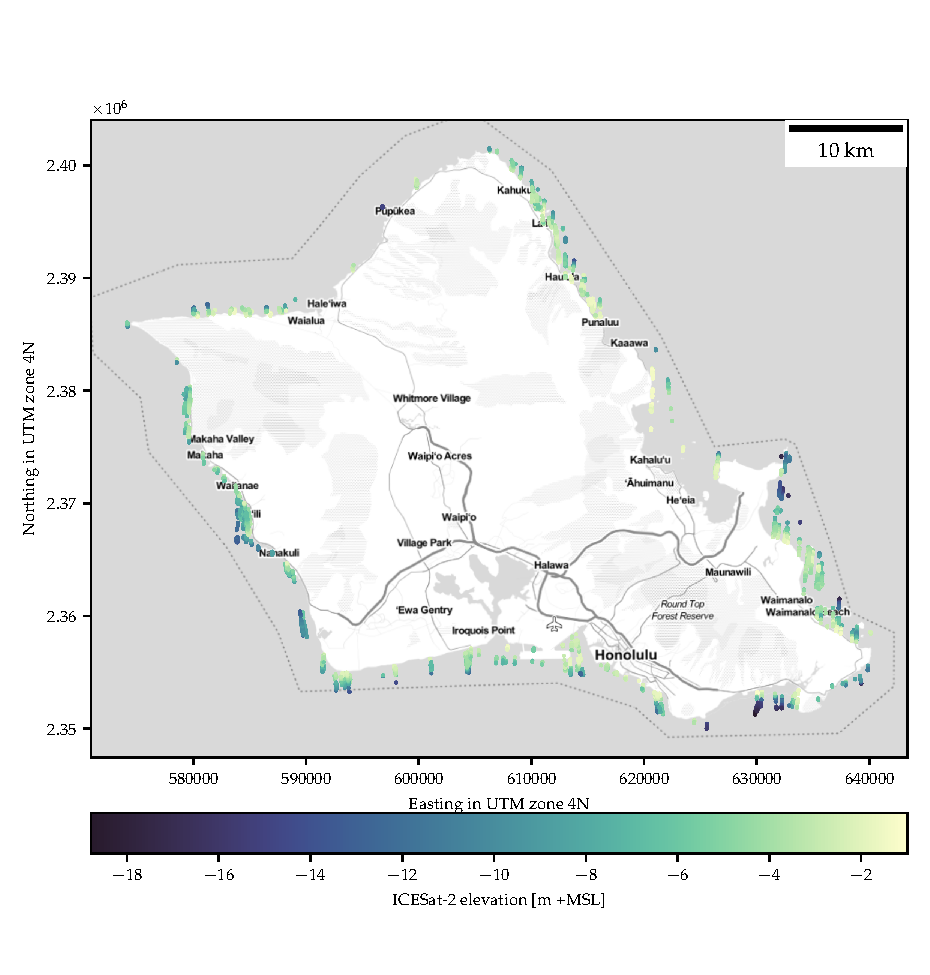
\includegraphics[width=\textwidth]{figures/Oahu_all_sites_photon_points.pdf}
%     \caption{The layout of the identified bathymetry point measurements around Oahu}
%     \label{fig:oahu-all-photon-map}
% \end{figure}

% The sites varied significantly in in the accuracy of the ICESat-2 point bathymetry. Some sites showed a significant RMS error due to the presense of mountain peaks up to a few hundred meters high with small horizontal footprint. These features are not captured by the GEBCO grid and therefore photon returns below them are not filtered due to the GEBCO-based horizontal filtering. Table \ref{table:Oahusitestats} contains the compiled error metrics for each site.

% \pdfcomment{add to discussion section} \pdfcomment{good to explain with a figure I think}

% \begin{table}[h!]
\caption{Error metrics between ICESat-2 and ground-truth data for all sites in Oahu}
\label{tab:Oahusitestats}
\begin{tabular}{lrrr}
\toprule
 & RMSE & MAE & Count bathy Points Identified \\
Oahu site number &  &  &  \\
\midrule
1 & 1.162525 & 0.768264 & 12775 \\
2 & 10.598899 & 1.447226 & 4327 \\
3 & 1.235144 & 0.463879 & 18566 \\
4 & 0.751631 & 0.565673 & 2738 \\
5 & 0.734813 & 0.504969 & 10443 \\
6 & 2.422447 & 1.756412 & 754 \\
7 & 1.111055 & 0.717672 & 2949 \\
8 & 0.670030 & 0.520755 & 17946 \\
\bottomrule
\end{tabular}
\end{table}


% The overall bias plot showing all the subsites is shown in figure \ref{fig:oahu-all-bias-plot}

% \begin{figure}[h]
%     \centering
%     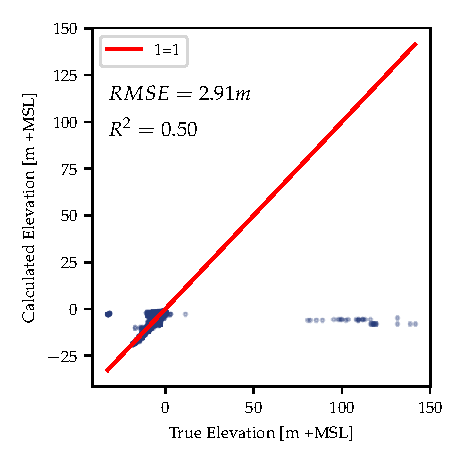
\includegraphics[width=0.7\textwidth]{figures/Oahu_combined_lidar_estimated_vs_truth.pdf}
%     \caption{Bias plot for all Oahu subsites combined}
%     \label{fig:oahu-all-bias-plot}
% \end{figure}

% The reason the RMSE at site 2 is much higher than the rest is that there was a mountain of 120m tall that was in the validation data. If that is removed, the error drops significantly. \pdfcomment{outlier rejection might be a fix for that.}
% \pdfcomment{these two figures could be combined into subplots probably }
% \begin{figure}[h]
%     \centering
%     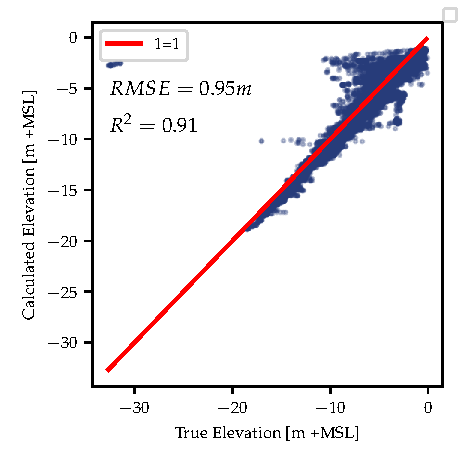
\includegraphics[width=0.7\textwidth]{figures/Oahu_combined_mountains_removed_lidar_estimated_vs_truth.pdf}
%     \caption{Oahu - all sites with mountain removed}
%     \label{fig:oahu-bias-no-mountains}
% \end{figure}

% To better show the distribution of the error smaller errors, figure \ref{fig:oahu-bias-no-mountains} shows the same combination of points, but with the outlier values 

% \subsection{Kalman Updating}



% \section{Summary}
% The results of all the test sites that used lidar data were combined into a single bias plot shown in figure \ref{fig:all-sites-biasplot}

% \subsection{ICESat-2 error}

% \begin{figure}[h]
%     \centering
%     \includegraphics[width=0.7\textwidth]{figures/all_site_combined_biasplot.pdf}
%     \caption{All lidar points for all sites with validation data}
%     \label{fig:all-sites-biasplot}
% \end{figure}

